After applying the HF scale factors derived in the previous subsection, a kinematic reweighitng is derived using a neural network. The kinematic reweighting is based on estimating a probability density function (p.d.f.) in an n-dimensional space by using a feed-forward classification neural network~\cite{nn_pdfs}. The output of a neural network trained to disentangle between two classes has a probabilistic interpretation in terms of the a-posteriori Bayesian probability. This can be used to approximate p.d.f. of the both class.

\begin{equation}
  o^{min}({\bf x}) = P(data|{\bf x}) = \dfrac{\alpha_{data}P_{data}({\bf x})}{\alpha_{data}P_{data}({\bf x})+\alpha_{MC}P_{MC}({\bf x})}
\end{equation}

where $o$ is NN output, ${\bf x}$ is input vector, $\alpha_{data}$ and $\alpha_{MC}$ are the proportions of each class of events used for training, satisfying $\alpha_{data} + \alpha_{MC} = 1$.

From the above equation, it is straightforward to extract reweighting factor as a ratio of two p.d.f.

\begin{equation}
  w({\bf x}) = \dfrac{\alpha_{data}P_{data}({\bf x})}{\alpha_{MC}P_{MC}({\bf x})} = \dfrac{o({\bf x})}{1-o({\bf x})}
  \label{rew::1l}
\end{equation}

Therefore the reweighting can be derived in ${\bf x}$ space for each event in an unbinned way. The both data and MC here refering to $\ttbar +jets$. To subtract non-\ttbar MC samples from the data, non-\ttbar MC samples are included in to the training with a data label, but by using a negative event weight. Then the final expression is still valid in the same form.

The training region is defined in $7j (5j)$ and $2b$ for 1L (2LOS). The neural network is fed by each jet $p_T$, number of jets and reclustered jets, missing $E_T$ and lepton jet $p_T$. The goal here is not only correcting these kinematics but also the kinematics derived from them.

With respect to all of the above, we modified loss function with an exponential loss function, therefore, reweighting factor is defined differently.
The motivation of this modification is due to some studies showing better performance especially in the case of low statistics~\cite{moustakides2019training}.


\begin{equation}
  \mathcal{L} = P_{data}e^{-o({\bf x})/2}+P_{MC}e^{o({\bf x})/2} \\
  \dfrac{d\mathcal{L}}{do({\bf x})} = -\dfrac{P_{data}}{2}e^{-o({\bf x})/2}+\dfrac{P_{MC}}{2}e^{o({\bf x})/2} = 0
\end{equation}

from this equation, reweighting factor can be derived as following,

\begin{equation}
  w({\bf x}) = e^{o({\bf x})}
\end{equation}

In addition to changing loss function, learning rate decay has been used during the training, and an early stop mechanism developed based on the minimization of loss function after each epoch.

Training has been performed on the \ttbar+jets nominal and alternative samples independently. So each sample was corrected by their own training. A generic feed-forward architecture found by a hyper-parameter scan for all trainings.

The kinematic reweighting on $H_T$ distribution is illusturated in Figure~\ref{fig::cor1l}. More discussion in Appendices~\ref{app:background_modeling_comp} and \ref{app:NNRewPlots}. It is expected that the kinematic reweighting does not change the normalization, only the shape. This was verified in Table~\ref{tab:Rew_NoRew_YieldsRatio}.

\begin{itemize}
\item Minimizer : Stochastic Gradient Descent
\item Learning Rate : 0.0036 and Momentum : 0.9
\item Loss function : Binary cross entropy / exponential
\item Architecture : 4ReLU(30)xTanh(30)xLinear(1)
\item Mini Batch size : 1000
\item Epoch : early stopping around 250 epoch
\end{itemize}

\begin{figure}[!htb]
  \centering
    \begin{subfigure}[t]{\textwidth}
        \centering
        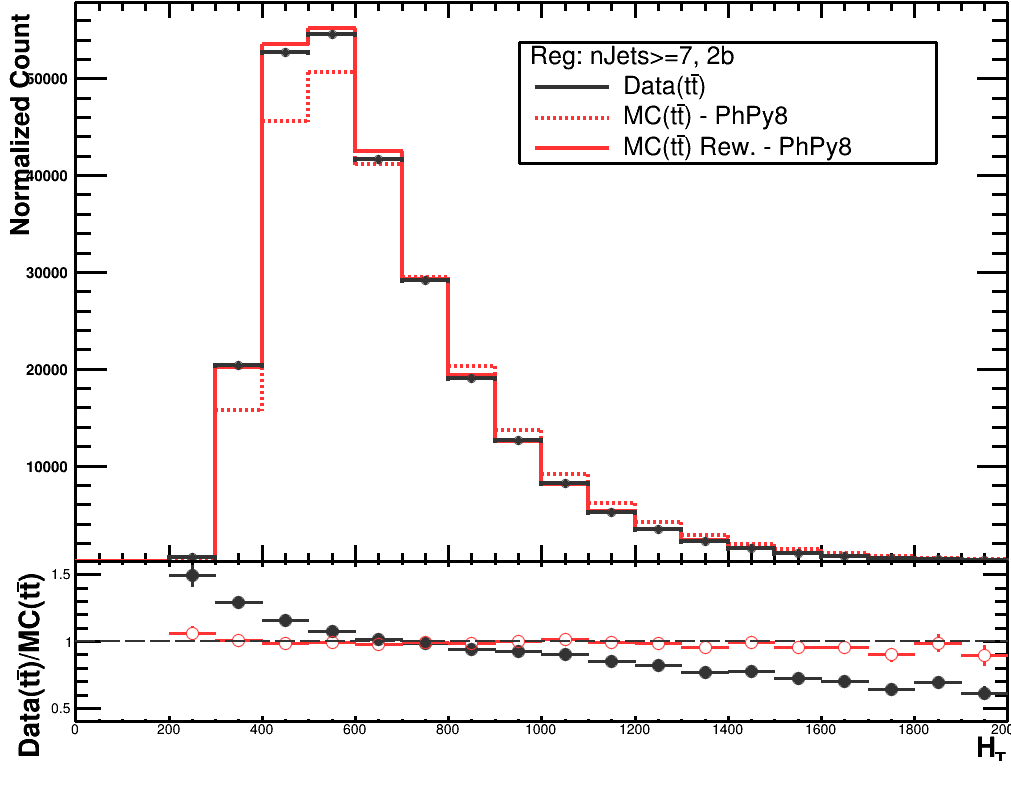
\includegraphics[width=0.48\textwidth]{plots/bkg_modelling/cor_1l_nom.png}
        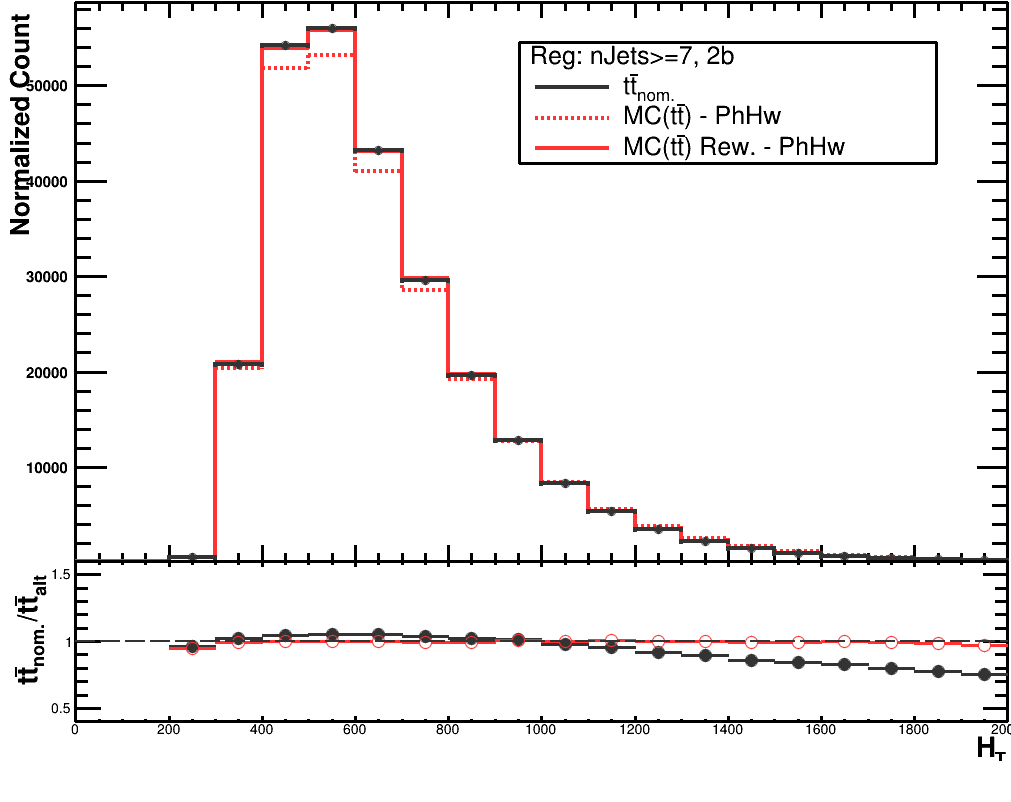
\includegraphics[width=0.48\textwidth]{plots/bkg_modelling/cor_1l_alt.png}
    \end{subfigure}
    \caption{The kinematic reweighting effect on $H_T$ distribution, and data/MC ratio for 1L \ttbar+jets nominal and one of the alternative samples. The black points in the ratio plot refer to data/MC ratio for the nominal MC samples with HF reweighting but without kinematic reweighting. The red points of the ratio plot refer to the data/MC ratio for the nominal MC samples after both HF and kinematic reweighting have been applied.}
    \label{fig::cor1l}
\end{figure}


\subsubsection{Uncertainty Propagation for NN Reweighting}
\label{sec:NN_reweighting:uncertainty}

Two additional uncertainties are considered to take into account the uncertainty on the data-driven
corrections. The reweighting factors on \ttbar + jets depend on the size of the non-\ttbar processes subtracted from data.
The cross section of the non-\ttbar processes is therefore varied by $\pm 50\%$ and alternative reweighting
factors are derived. The resulting difference in the final distribution is taken as a nuisance parameter in the
likelihood fit. The effect of this uncertainty ranges from 3\% to 4\%.

Understanding the influence of statistical uncertainty on background modeling aids in calibrating adjustments to the data within the fitted distributions.
Among the array of available methods in the literature, the Monte Carlo (MC) dropout method~\cite{gal2016dropout} was selected for its straightforward implementation and its flexibility in 
accommodating diverse neural network architectures. The dropout is originally a regularization method for neural networks where randomly selected neurons are ignored during training.
To apply this method following steps are considered,

\begin{itemize}
    \item {\bf Standard training:} Initialy a neural network is trained for reweighting factors without implementation of dropout layers.
    \item {\bf Dropout training:} A second training is considered with implementation of dropout layers into same architecture of standard training.
    \item {\bf Dropout evaluation:} The neural network from the dropout training is evaluated 1000 times by keep using dropout layers, so the random drops of neurons still remain, and results varied up in each iteration.
    \item {\bf Uncertainty propagation:} The standard deviation is calculated from the varied results of dropout evaluation. 
\end{itemize}


This method has been tested via toy and real data to understand better to effect of statistics on uncertainty.
For this example, we have created two different exponential distributions and matched them to each other through the neural network reweighting, and a fit function.
The uncertainty from the MC dropout method and the confidence interval at 68\% from the fit are compared in Figure~\ref{fig::unc_rew}, for poor and high statistics.
A similar test has been done on the training region by selecting different multiplicity of number of jets to observe how statistical fluctuation is effecting on this method in Figure~\ref{fig::unc_rew_real}

\begin{figure}[!htb]
    \centering
      (a)
      \begin{subfigure}[t]{\textwidth}
          \centering
          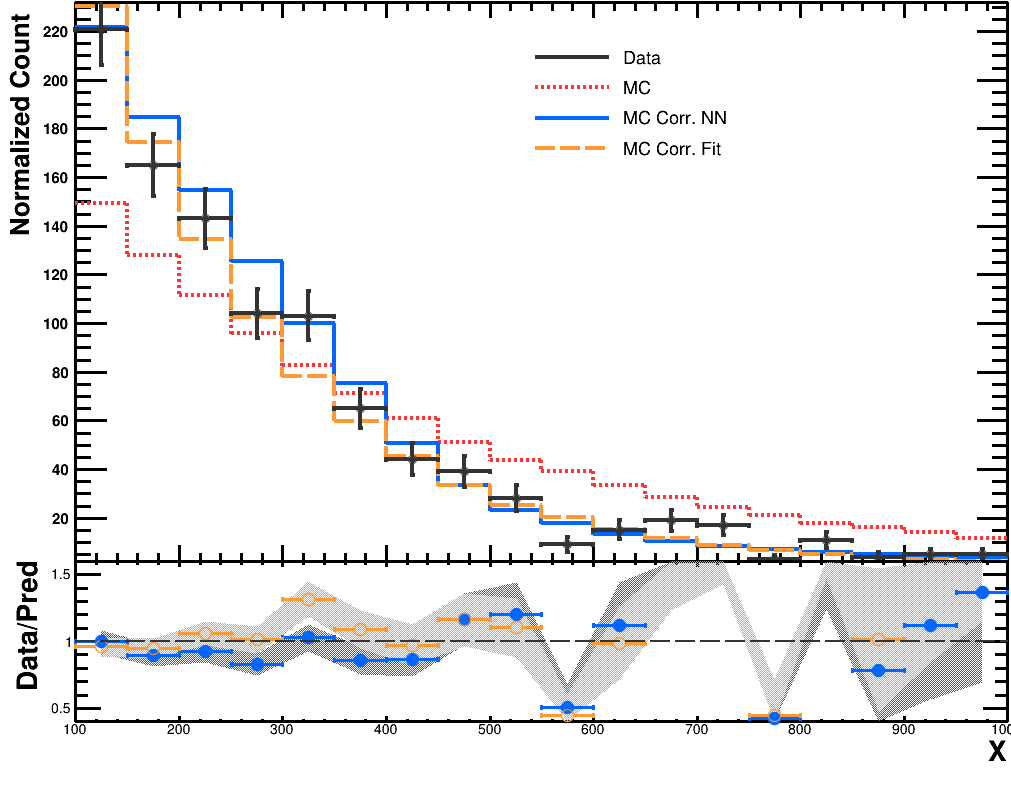
\includegraphics[width=0.48\textwidth]{plots/bkg_modelling/toy_poor.png}
          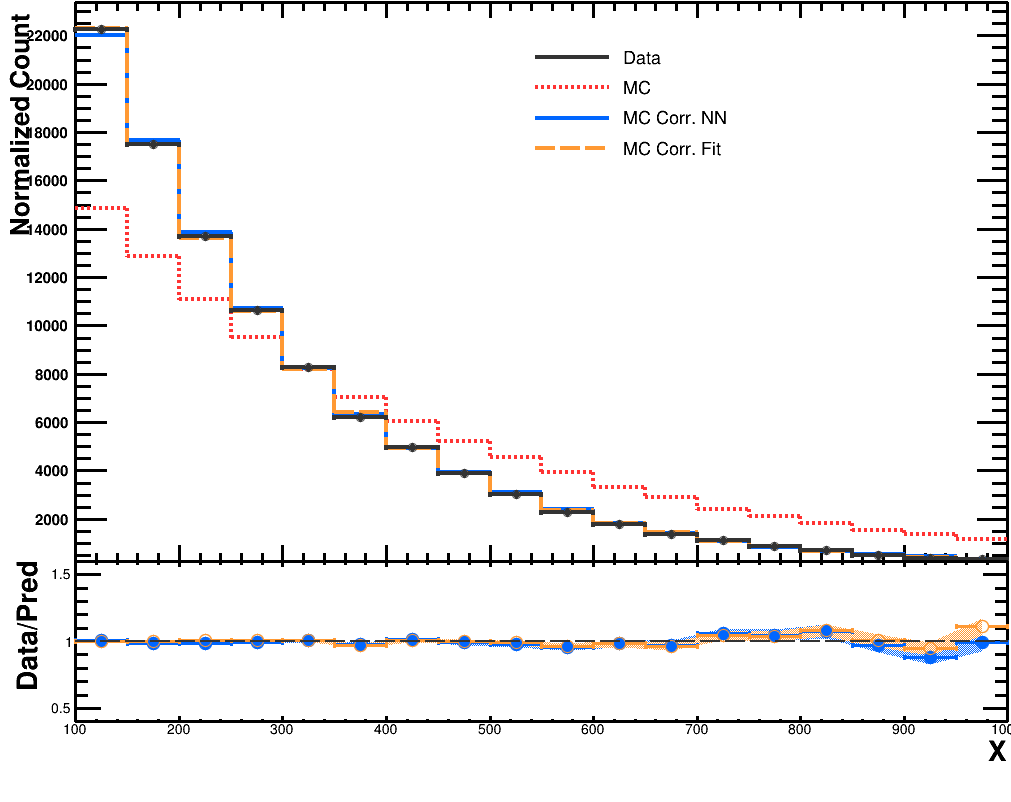
\includegraphics[width=0.48\textwidth]{plots/bkg_modelling/toy.png}
      \end{subfigure}
      (b)
      \begin{subfigure}[t]{\textwidth}
        \centering
        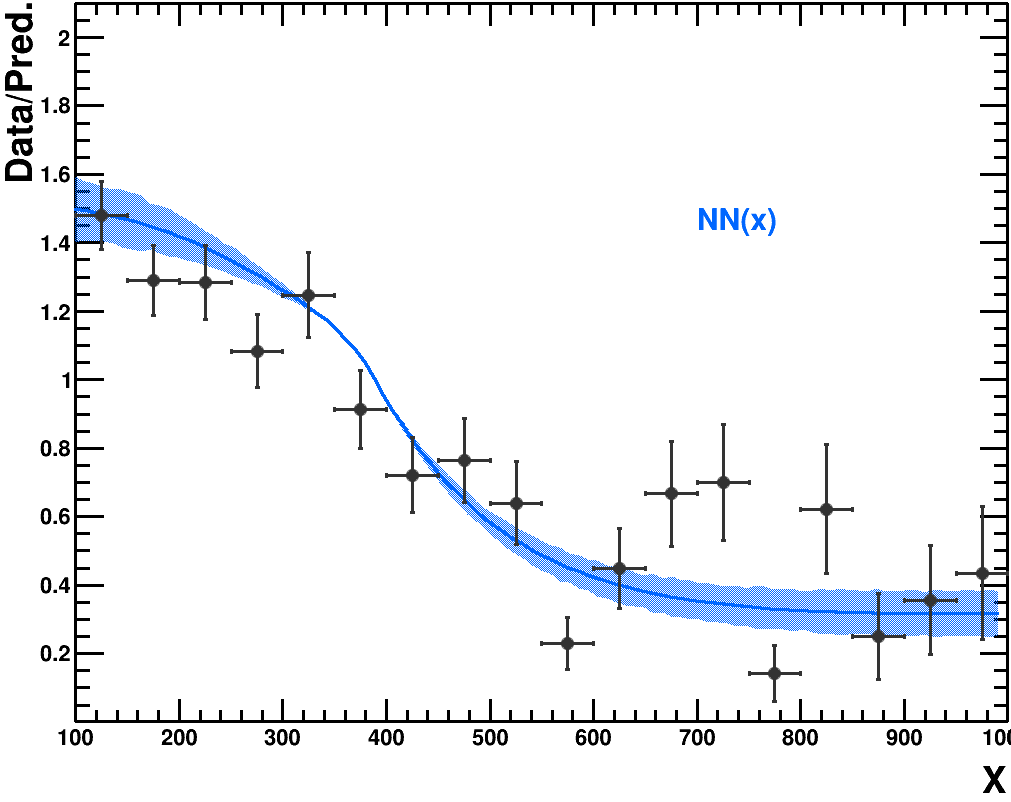
\includegraphics[width=0.48\textwidth]{plots/bkg_modelling/toy_nn_poor.png}
        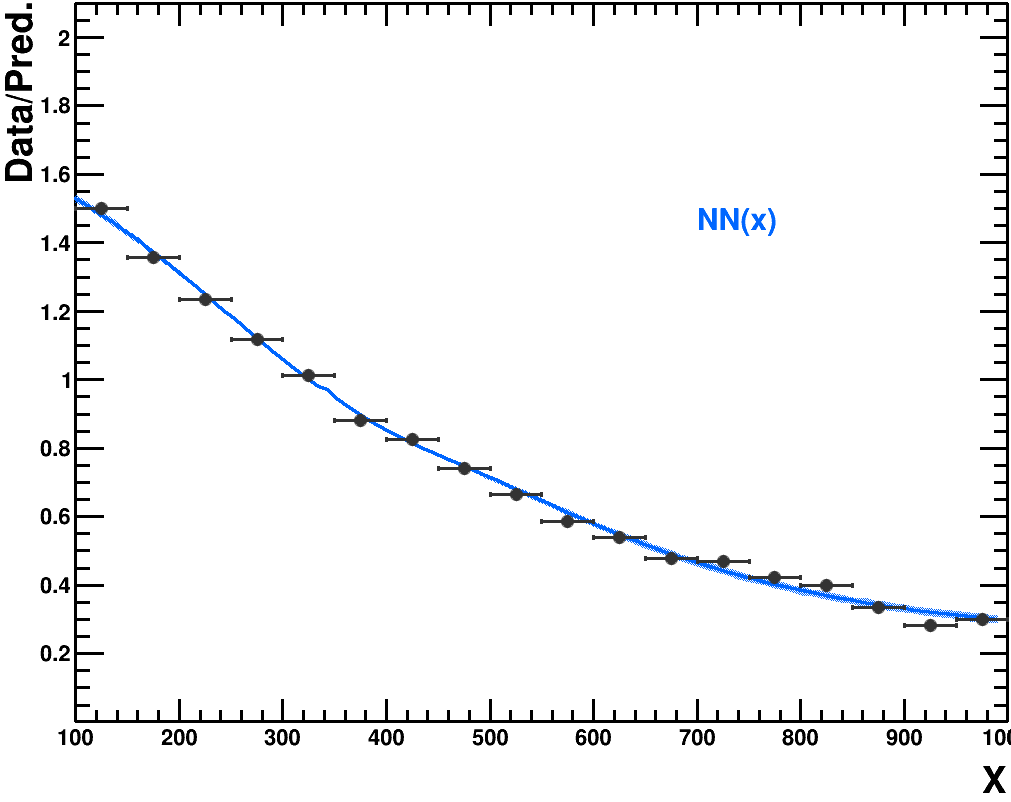
\includegraphics[width=0.48\textwidth]{plots/bkg_modelling/toy_nn.png}
      \end{subfigure}
      (c)
      \begin{subfigure}[t]{\textwidth}
        \centering
        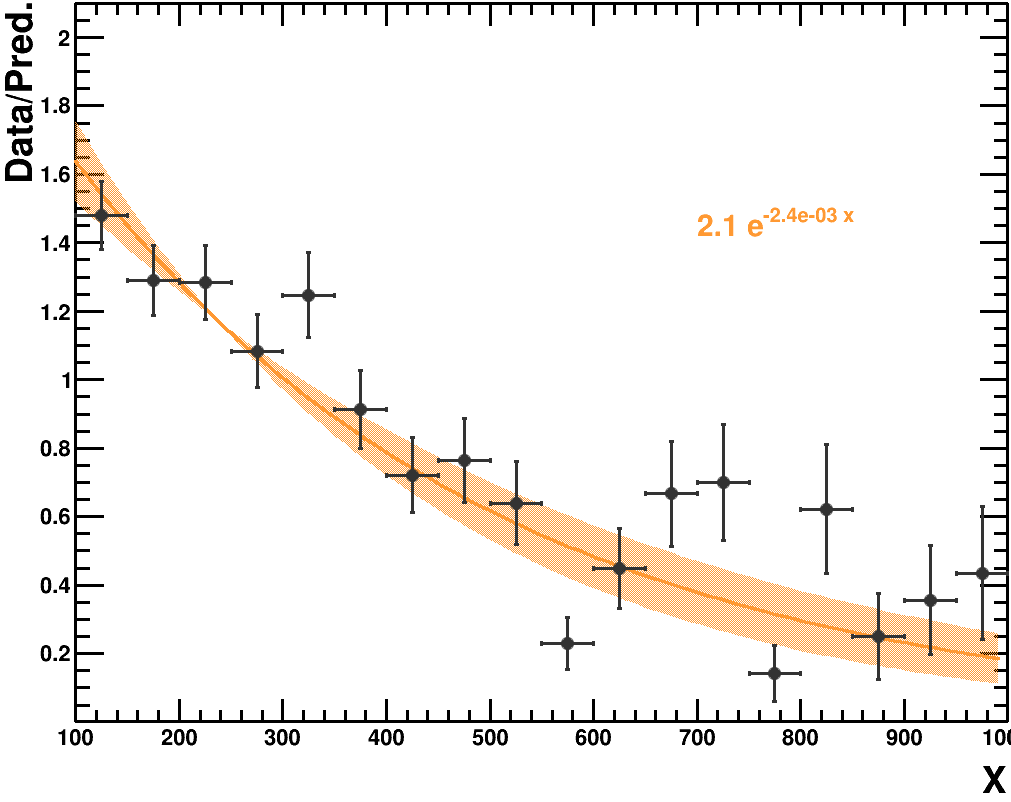
\includegraphics[width=0.48\textwidth]{plots/bkg_modelling/toy_fit_poor.png}
        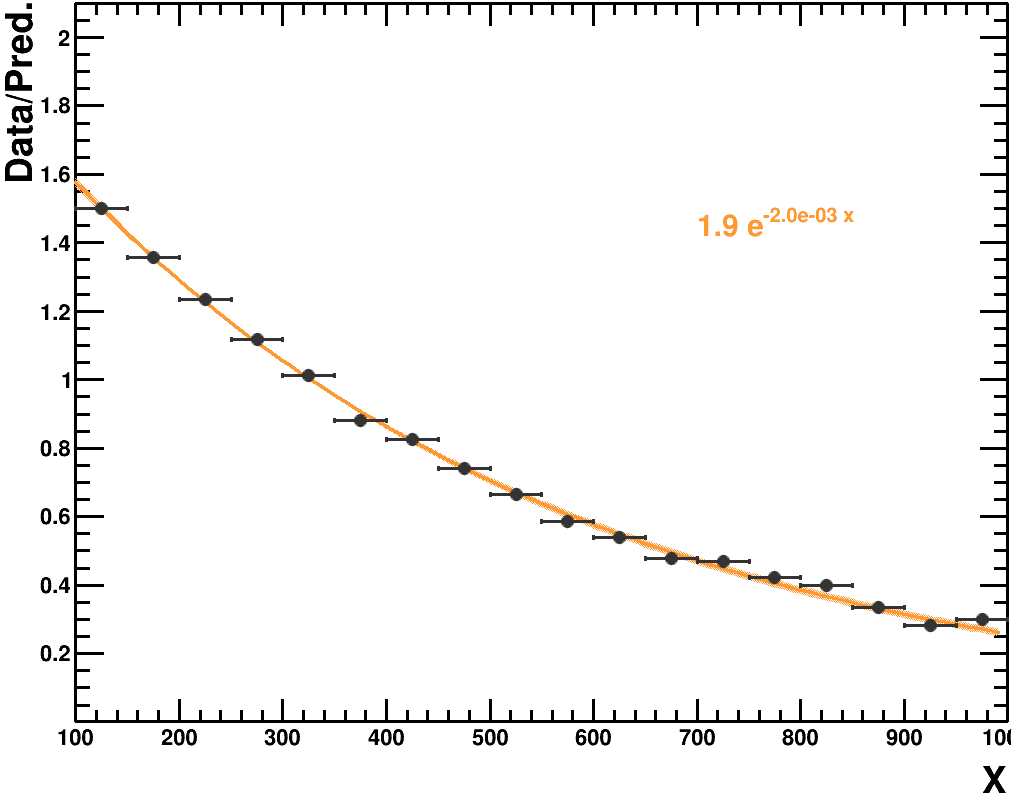
\includegraphics[width=0.48\textwidth]{plots/bkg_modelling/toy_fit.png}
      \end{subfigure}
     \caption{A toy example, generated randomly with two different coefficients of exponential function labeled as data and MC for 1000 (left), and 100000 (right) events.
     (a) Showing correction from NN reweighting and fit function with their uncertainty, (b) reweighting function from NN training and derived uncertainty,
     (c) fit function and the confidence interval at 68\%}
      \label{fig::unc_rew}
  \end{figure}

The given example in Figure~\ref{fig::unc_rew} shows a comparable effect of statistical error on the both NN, and fit modeling for background estimation. Therefore, the statistical errors on the derived reweighting factors are propagated through the MC dropout method, to the \ttbar +jets prediction and their impact are considered as nuisance parameters in the likelihood fit.

\begin{figure}[!htb]
    \centering
      (a)
      \begin{subfigure}[t]{\textwidth}
          \centering
          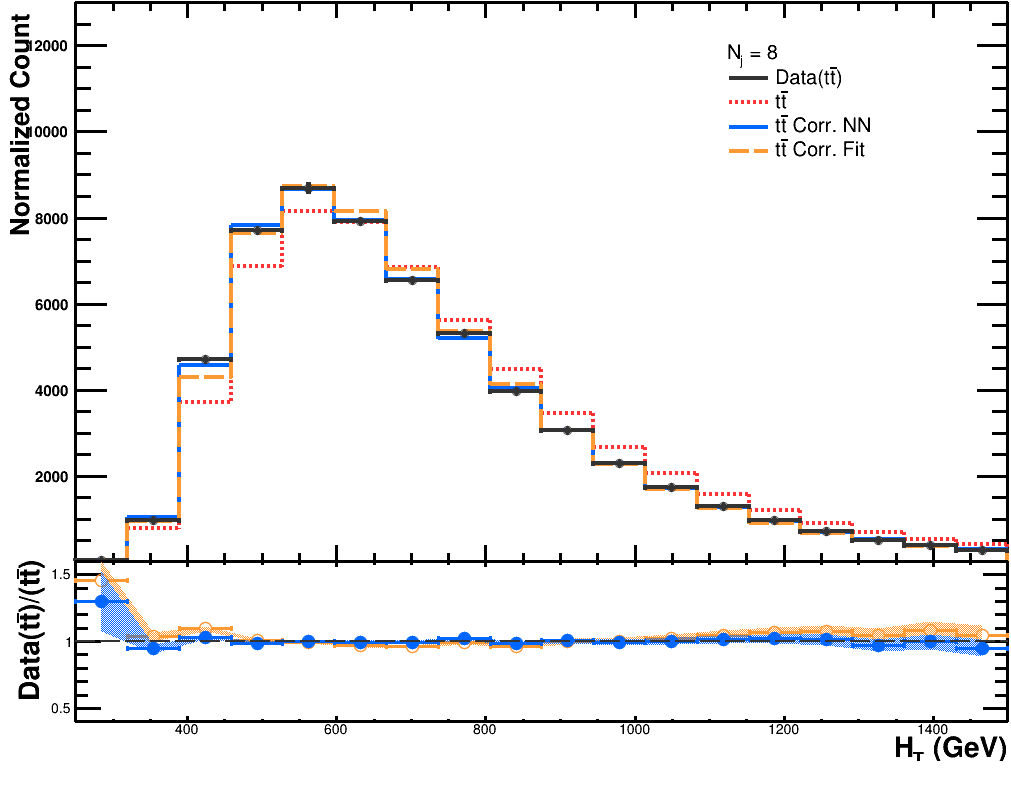
\includegraphics[width=0.48\textwidth]{plots/bkg_modelling/nn_rew_unc_real/val_8.png}
          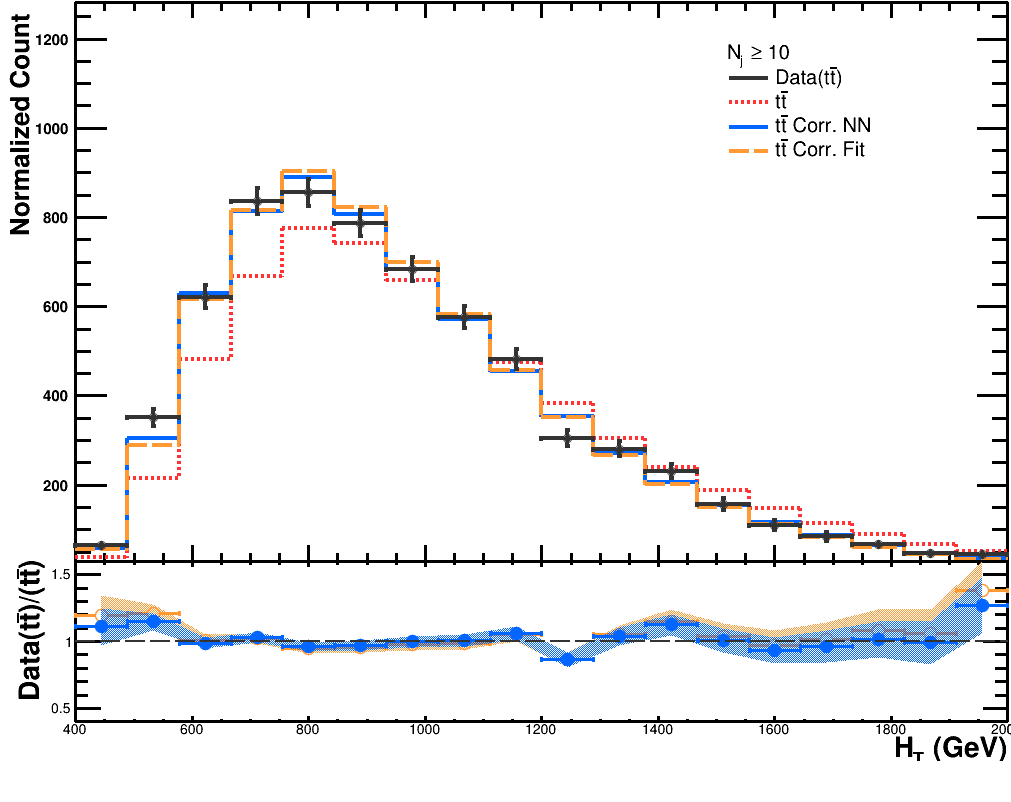
\includegraphics[width=0.48\textwidth]{plots/bkg_modelling/nn_rew_unc_real/val_geq10.png}
      \end{subfigure}
      (b)
      \begin{subfigure}[t]{\textwidth}
        \centering
        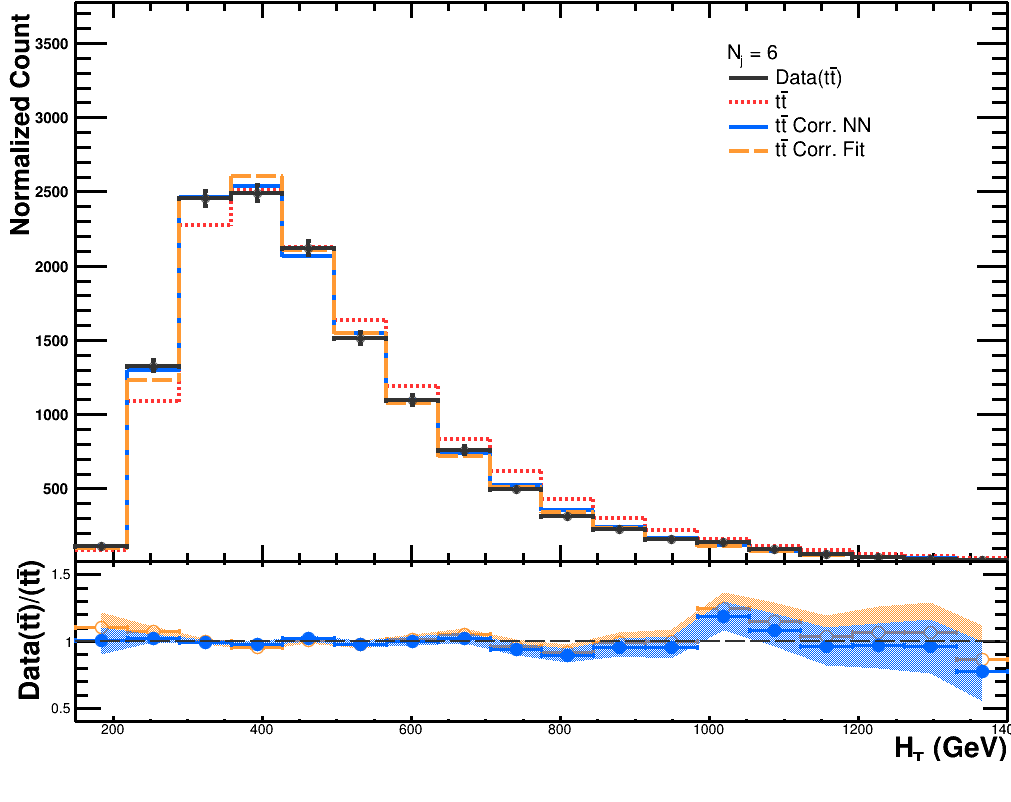
\includegraphics[width=0.48\textwidth]{plots/bkg_modelling/nn_rew_unc_real/val_2los_6.png}
        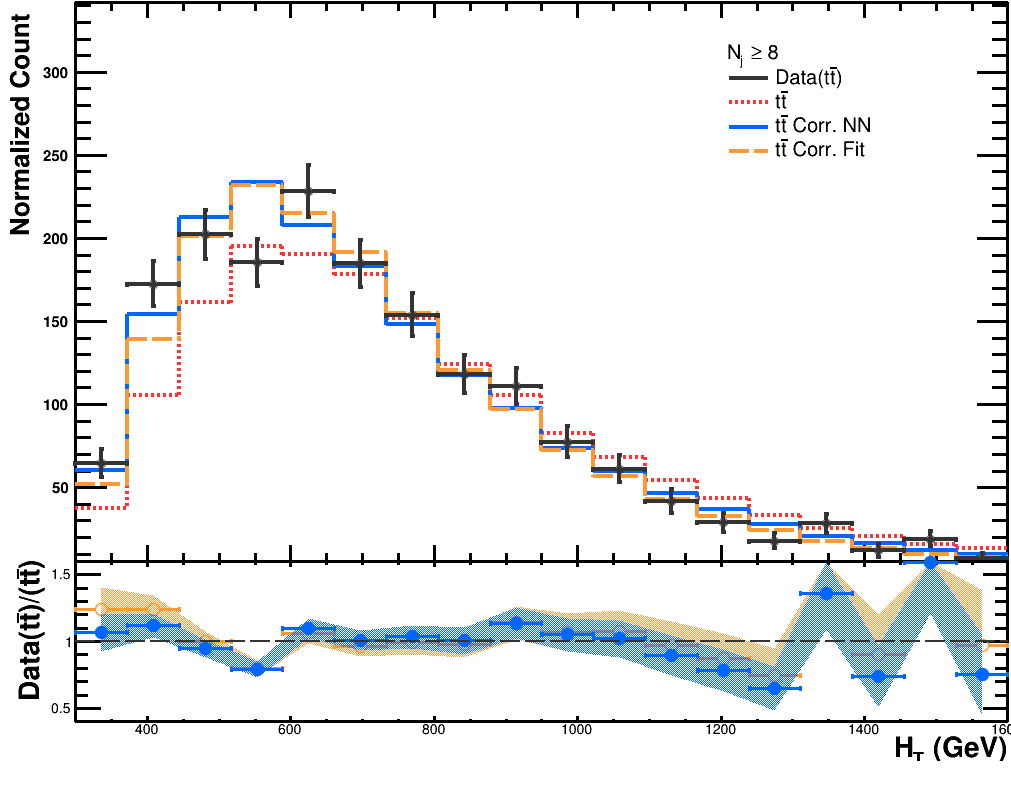
\includegraphics[width=0.48\textwidth]{plots/bkg_modelling/nn_rew_unc_real/val_2los_geq8.png}
      \end{subfigure}
     \caption{$H_{T}$ distributions with data/MC ratio for before and after correction from NN reweighting and MC dropout method, and fit modeling from two different coefficients of exponential function, and its confidence interval at 68\% (a) 1L, (b) (2LOS) channel, and left exclusive 8j(6j), right at least 10j(8j) jets multiplicities selections.}
      \label{fig::unc_rew_real}
  \end{figure}
